\documentclass{beamer}

\usepackage[utf8]{inputenc}
\usepackage[T1]{fontenc}
\usepackage{booktabs}
\usepackage[scale=2]{ccicons}
\usepackage{pgfplots}
\usepgfplotslibrary{dateplot}
\usepackage{xspace}
\usepackage{pbox}

% a few macros
\newcommand{\bi}{\begin{itemize}}
\newcommand{\ei}{\end{itemize}}
\newcommand{\be}{\begin{enumerate}}
\newcommand{\ee}{\end{enumerate}}
\newcommand{\ig}{\includegraphics}
\definecolor{hilight}{RGB}{235,129,27}
\definecolor{vhilight}{RGB}{235,129,27}
\definecolor{title}{RGB}{107,174,214}
\definecolor{subtitle}{RGB}{102,255,204}


% Tikz
\usepackage{tikz}
\usetikzlibrary{arrows,shapes}

% Minted
\usepackage{minted}
\usemintedstyle{manni}
\newminted{cpp}{fontsize=\footnotesize}

% Graph styles
\tikzstyle{vertex}=[circle,fill=black!50,minimum size=15pt,inner sep=0pt, font=\small]
\tikzstyle{selected vertex} = [vertex, fill=red!24]
\tikzstyle{edge} = [draw,thick,-]
\tikzstyle{dedge} = [draw,thick,->]
\tikzstyle{weight} = [font=\scriptsize,pos=0.5]
\tikzstyle{selected edge} = [draw,line width=2pt,-,red!50]
\tikzstyle{ignored edge} = [draw,line width=5pt,-,black!20]

\tikzset{
  treenode/.style = {align=center, inner sep=0pt, text centered,
    font=\sffamily},
  vertex/.style = {treenode, circle, black, font=\sffamily\bfseries\tiny, draw=black, text width=1.8em},% arbre rouge noir, noeud noir
  rvertex/.style = {treenode, circle, black, font=\sffamily\bfseries\tiny, draw=red, text width=1.8em},% arbre rouge noir, noeud noir
}

%Information to be included in the title page:
\title[]{Presentasi}
\author[Carles]{Carles Octavianus}
\date{2022}

\begin{document}

\frame{\titlepage}

\begin{frame}[fragile]
    \frametitle{Table of Contents}
    \tableofcontents
\end{frame}


\section{Nomor 1 Python}
\begin{frame}{Ide Pengerjaan}
    \begin{itemize}
        \item mengubah list busur (variable ROUTES) menjadi list ketetangaan \pause
        \item melakukan breath first search dari node start pada graph (list ketetangaan) tersebut. \pause
        \item Breadth-first search akan bergerak ke node berikutnya sesuai dengan kenaikan jaraknya (relatif terhadap node start) \pause
        \item dengan begitu, single breadth-first search dari start ke end akan menjamin lintasan tersebut adalah lintasan terpendeknya. \pause
        \item selama proses BFS kita bisa mencatat jarak relatif node lain terhadap node start.
    \end{itemize}
\end{frame}

\begin{frame}[fragile]{List Busur}
    \begin{columns}
    \column{0.5\textwidth}
    \begin{minted}{python}
    ROUTES=[[0,1],[0,2],[1,2],[2,3]]
    \end{minted}
    
    \column{0.5\textwidth}
    
    \begin{figure}
                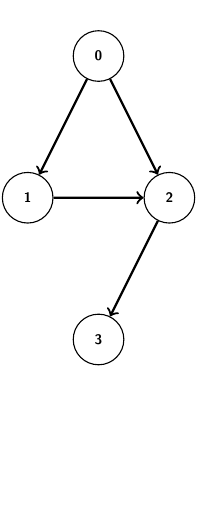
\begin{tikzpicture}[scale=1.8,auto,swap]
                    
                        \node[vertex] (0) at (0.5,3) {0};
                        \node[vertex] (1) at (0,2) {1};
                        \node[vertex] (2) at (1,2) {2};
                        \node[vertex] (3) at (0.5,1) {3};
                    
                    
                        \path[dedge] (0) -- (1);
                        \path[dedge] (0) -- (2);
                        \path[dedge] (1) -- (2);
                        \path[dedge] (2) -- (3);
                    
                    \pgfresetboundingbox
                    \path [use as bounding box] (0,0) rectangle (1,3.2);
                \end{tikzpicture}
            \end{figure}
    \end{columns}
\end{frame}
\begin{frame}[fragile]{List Ketetangaan}
 \begin{columns}[T]
        \begin{column}{.4\textwidth}
            \begin{minted}{python}
0: 1,2
1: 2
2: 3
3:

    adj=defaultdict(list)
    for u,v in ROUTES:
        adj[u]+=[v]
            \end{minted}
        \end{column}%
        \hfill%
        \begin{column}{.4\textwidth}
            \ \begin{figure}
                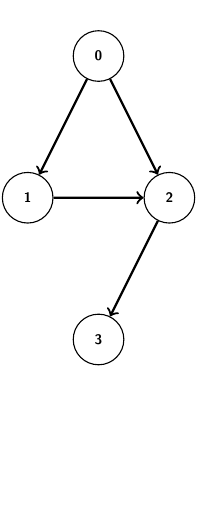
\begin{tikzpicture}[scale=1.8,auto,swap]
                    
                        \node[vertex] (0) at (0.5,3) {0};
                        \node[vertex] (1) at (0,2) {1};
                        \node[vertex] (2) at (1,2) {2};
                        \node[vertex] (3) at (0.5,1) {3};
                    
                    
                        \path[dedge] (0) -- (1);
                        \path[dedge] (0) -- (2);
                        \path[dedge] (1) -- (2);
                        \path[dedge] (2) -- (3);
                    
                    \pgfresetboundingbox
                    \path [use as bounding box] (0,0) rectangle (1,3.2);
                \end{tikzpicture}
            \end{figure}
        \end{column}%
    \end{columns}
\end{frame}

\begin{frame}{Breadth-first search}
  \begin{figure}
    \begin{tikzpicture}[auto, swap]
      \node[vertex] (0) at (-0.3,2) {0};
      \node[vertex] (1) at (0.0,-0.5) {1};
      \node[vertex] (2) at (1.9,0.7) {2};
      \node[vertex] (3) at (2.4,2.7) {3};
      \node[vertex] (4) at (3.4,-0.8) {4};
      \node[vertex] (5) at (3.9,1) {5};
      \node[vertex] (6) at (6.2,1.1) {6};
      \node[vertex] (7) at (6.1,-0.9) {7};
      \node[vertex] (8) at (5.7,3.2) {8};
      \node[vertex] (9) at (8.3,2.1) {9};
      \node[vertex] (10) at (8.1,0.1) {10};

      \path[dedge] (0) -- (1);
      \path[dedge] (0) -- (2);

      \path[dedge] (1) -- (4);

      \path[dedge] (2) -- (1);
      \path[dedge] (2) -- (3);

      \path[dedge] (3) -- (0);

      \path[dedge] (4) -- (5);

      \path[dedge] (5) -- (2);
      \path[dedge] (5) -- (3);
      \path[dedge] (5) -- (6);
      \path[dedge] (5) -- (7);
      \path[dedge] (5) -- (8);

      %\path[dedge] (6) -- (5);
      \path[dedge] (6) -- (8);
      \path[dedge] (6) -- (7);

      %\path[dedge] (8) -- (5);
      \path[dedge] (8) to [bend left] (9);

      \path[dedge] (9) to [bend left] (8);

      \path[dedge] (7) -- (10);

      \only<2-4>{\node[vertex,fill=vhilight] (0) at (-0.3,2) {0};}
      \only<3-4>{
        \path[dedge,vhilight] (0) -- (1);
        \path[dedge,vhilight] (0) -- (2);
      }

      \only<5->{\node[vertex,fill=title] (0) at (0) {0};}
      \only<5->{\path[dedge,thick,title] (0) -- (1);}
      \only<5->{\path[dedge,thick,title] (0) -- (2);}
      \only<5->{\node[vertex,fill=vhilight] (1) at (1) {1};}

      \only<6-7>{\path[dedge,vhilight] (1) -- (4);}
      \only<8->{\path[dedge,thick,title] (1) -- (4);}

      \only<8->{\node[vertex,fill=title] (1) at (1) {1};}
      \only<8-10>{\node[vertex,fill=vhilight] (2) at (2) {2};}
      \only<9-10>{\path[dedge,vhilight] (2) -- (3);}
      \only<8-10>{\node[vertex,fill=vhilight] (2) at (2) {2};}


      \only<10>{\path[dedge,vhilight] (2) -- (3);}
      \only<11->{\node[vertex,fill=title] (2) at (2) {2};}
      \only<11->{\path[dedge,title,thick] (2) -- (3);}
      \only<11-13>{\node[vertex,fill=vhilight] (4) at (4) {4};}
      \only<12-13>{\path[dedge,vhilight] (4) -- (5);}

      \only<14->{\node[vertex,fill=title] (4) at (4) {4};}
      \only<14->{\path[dedge,thick,title] (4) -- (5);}
      \only<14>{\node[vertex,fill=vhilight] (3) at (3) {3};}

      \only<14>{\node[vertex,fill=vhilight] (3) at (3) {3};}
      \only<15->{\node[vertex,fill=title] (3) at (3) {3};}

      \only<15-17>{\node[vertex,fill=vhilight] (5) at (5) {5};}
      \only<16-17>{
        \path[dedge,vhilight] (5) -- (6);
        \path[dedge,vhilight] (5) -- (7);
        \path[dedge,vhilight] (5) -- (8);
      }
      \only<18->{
        \node[vertex,fill=title] (5) at (5) {5};
        \path[dedge,title,thick] (5) -- (6);
        \path[dedge,title,thick] (5) -- (7);
        \path[dedge,title,thick] (5) -- (8);
      }
      \only<18>{ \node[vertex,fill=vhilight] (6) at (6) {6}; }
      \only<19->{ \node[vertex,fill=title] (6) at (6) {6}; }

      \only<19-21>{ \node[vertex,fill=vhilight] (7) at (7) {7}; }
      \only<20-21>{\path[dedge,vhilight] (7) -- (10);}

      \only<22->{ 
        \node[vertex,fill=title] (7) at (7) {7};
        \path[dedge,title,thick] (7) -- (10);
      }

      \only<22-24>{\node[vertex,fill=vhilight] (8) at (8) {8};}
      \only<23-24>{\path[dedge,vhilight] (8) to[bend left] (9)};

      \only<25->{
        \node[vertex,fill=title] (8) at (8) {8};
        \path[dedge,title] (8) to[bend left] (9);
      }
      \only<25>{\node[vertex,fill=vhilight] (10) at (10) {10};}
      \only<26->{\node[vertex,fill=title] (10) at (10) {10};}
      \only<26>{\node[vertex,fill=vhilight] (9) at (9) {9};}
      \only<27->{\node[vertex,fill=title] (9) at (9) {9};}

    \end{tikzpicture}
  \end{figure}

  %\mintinline{cpp}{Queue: }
  \texttt{ \begin{tabular}{l l}
  \texttt{Queue: } & 
   \only<2-3>{{\color{vhilight}0}}\only<4>{{\color{vhilight}0} 1 2}\only<5-6>{{\color{vhilight}1} 2}\only<7>{{\color{vhilight}1} 2 4}\only<8-9>{{\color{vhilight}2} 4}\only<10>{{\color{vhilight}2} 4 3}\only<11-12>{{\color{vhilight}4} 3}\only<13>{{\color{vhilight}4} 3 5}\only<14>{{\color{vhilight}3} 5}\only<15-16>{{\color{vhilight}5}}\only<17>{{\color{vhilight}5} 6 7 8}\only<18>{{\color{vhilight}6} 7 8}\only<19-20>{{\color{vhilight}7} 8}\only<21>{{\color{vhilight}7} 8 10}\only<22-23>{{\color{vhilight}8} 10}\only<24>{{\color{vhilight}8} 10 9}\only<25>{{\color{vhilight}10} 9}\only<26>{{\color{vhilight}9}}
  \end{tabular}}

  \vspace{10pt}
  \texttt{
    \begin{tabular}{l | c c c c c c c c c c c }
      & 0 & 1 & 2 & 3 & 4 & 5 & 6 & 7 & 8 & 9 & 10 \\
      marked 
      & \only<1>{0}\only<2->{{\color{title}1}} 
      & \only<1-3>{0}\only<4->{{\color{title}1}} 
      & \only<1-3>{0}\only<4->{{\color{title}1}} 
      & \only<1-9>{0}\only<10->{{\color{title}1}} 
      & \only<1-6>{0}\only<7->{{\color{title}1}} 
      & \only<1-12>{0}\only<13->{{\color{title}1}} 
      & \only<1-16>{0}\only<17->{{\color{title}1}} 
      & \only<1-16>{0}\only<17->{{\color{title}1}} 
      & \only<1-16>{0}\only<17->{{\color{title}1}} 
      & \only<1-23>{0}\only<24->{{\color{title}1}}
      & \only<1-20>{0}\only<21->{{\color{title}1}} \\
    \end{tabular}}
\end{frame}

\section{Nomor 2 Mathematica}
\begin{frame}{Ide Pengerjaan}

Kita akan melakukan traversal pada grid dengan pergerakan spiral, 
lalu mengisi cell tersebut dengan angka dari $1$ sampai $n^2$. \pause

Tinjau bahwa, secara berurutan pergerakannya hanyalah $\{\downarrow, \rightarrow, \uparrow, \leftarrow\, \dots\}$. \pause
Kita hanya perlu kondisi kapan kita akan berganti gerakan (contoh: dari gerakan kebawah menjadi gerakan kekanan)
Tinjau beberapa kasus general berikut:
\end{frame}

\begin{frame}[fragile]{Kasus 1}
    \item 
    \begin{table}[!ht]
        \centering
        \caption{Kasus 1: mengganti gerakan ketika akan keluar dari grid-nya}
        \begin{tabular}{|l|l|l|l|}
        \hline
            1 & - & - & - \\ \hline
            2 & - & - & - \\ \hline
            3 & - & - & - \\ \hline
            X & - & - & - \\ \hline
        \end{tabular}
        \label{spiralgrid1}
    \end{table}

    Tinjau tabel \ref{spiralgrid1}. Pada kasus ini, kita sudah traverse kebawah hingga posisi X.
    untuk mengganti ke gerakan selanjutnya, kita gunakan conditional ketika gerakan awal (sebelum berganti) mengakibatkan posisi keluar dari grid.
    Dengan begitu, untuk contoh kasus di atas kita punya kondosi berikut:
   
\end{frame}

\begin{frame}[fragile]{Kasus 1 Cont}
     \begin{minted}{python}
IF posisi_baris+current_movement_baris>n
    current_movement_baris= next_movement_baris
    current_movement_kolom= next_movement_kolom
END IF
    \end{minted}
    Untuk ketiga kasus out of grid lainnya similar.
\end{frame}

\begin{frame}{Kasus 2}
    \begin{table}[!h]
        \centering
        \caption{mengganti gerakan ketika posisi selanjutnya sudah disi}
        \begin{tabular}{|l|l|l|l|}
        \hline
            1 & - & - & - \\ \hline
            2 & - & - & - \\ \hline
            3 & 10 & 9 & 8 \\ \hline
            4 & 5 & 6 & 7 \\ \hline
        \end{tabular}
        \label{spiralgrid2}
    \end{table}


    Tinjau tabel \ref{spiralgrid2}. pada kasus ini kita berada di posisi 10 dan sedang bergerak ke kiri.
    Tinjau bahwa jika kita bergerak ke kanan, sel selanjutnya sudahlah diisi. oleh karena itu,
    kita bisa mengganti gerakannya dengan kondisikondisi sel selanjutnya sudah diisi.
    dalam psudocode:
    
\end{frame}

\begin{frame}[fragile]{kasus 2 cont}
\small
\begin{minted}{python}

IF grid[posisi_baris+current_movement+baris]
[posisi_kolom+current_movement_kolom] not empty
current_movement_baris= next_movement_baris
current_movement_kolom= next_movement_kolom
END IF
\end{minted}
\end{frame}

\begin{frame}{Nomor 2 Mathematica}
Selanjutnya, Nilai terbesar selalulah $n^2$ dan posisinya akan ditengah jika $n$ ganjil.
lalu sumasi dari elemen pada grid adalah $1+2+\dots +n^2= \frac{n^2 (n^2+1)}{2}$
\end{frame}
\end{document}